% This is part of Un soupçon de mathématique sans être agressif pour autant
% Copyright (c) 2012-2013
%   Laurent Claessens, Pauline Klein
% See the file fdl-1.3.txt for copying conditions.

%+++++++++++++++++++++++++++++++++++++++++++++++++++++++++++++++++++++++++++++++++++++++++++++++++++++++++++++++++++++++++++
\section{Activité : mois de naissance}
%+++++++++++++++++++++++++++++++++++++++++++++++++++++++++++++++++++++++++++++++++++++++++++++++++++++++++++++++++++++++++++

Prendre les mois de naissance des élèves, en séparant les groupes.
\begin{enumerate}
    \item
        Quel groupe a la proportion de naissance en mars la plus grande ?
    \item
        En tout quelle est la proportion des naissances en avril ?
    \item 
        Est-ce qu'on peut voir l'effet comme quoi les mois de \( 31\) jours son plus longs ? 
        \begin{enumerate}
            \item
                Quelle est la proportion d'élèves nés dans un mois de \( 31\) jours ?
            \item
                Il y a \( 7\) mois de $31$ jours contre \( 5\) de moins. Donc le résultat est biaisé.
            \item
                Calculer la \emph{fréquence} des naissances en naissances par mois.
        \end{enumerate}
\end{enumerate}

%+++++++++++++++++++++++++++++++++++++++++++++++++++++++++++++++++++++++++++++++++++++++++++++++++++++++++++++++++++++++++++
\section{Regardons des graphiques}
%+++++++++++++++++++++++++++++++++++++++++++++++++++++++++++++++++++++++++++++++++++++++++++++++++++++++++++++++++++++++++++

Les graphiques sont souvent tirés de wikipédia. Si vous voulez plus d'informations, lisez \url{http://www.manicore.com/}, ou bien regardez le cours \href{http://www.mines-paristech.fr/ingenieurcivil/SitesIC/Balado/Climat_som.html}{en ligne}, en particulier la deuxième heure du troisième cours donne les facteurs d'émissions dans le monde et en France.

%---------------------------------------------------------------------------------------------------------------------------
\subsection{Émissions par secteurs}
%---------------------------------------------------------------------------------------------------------------------------

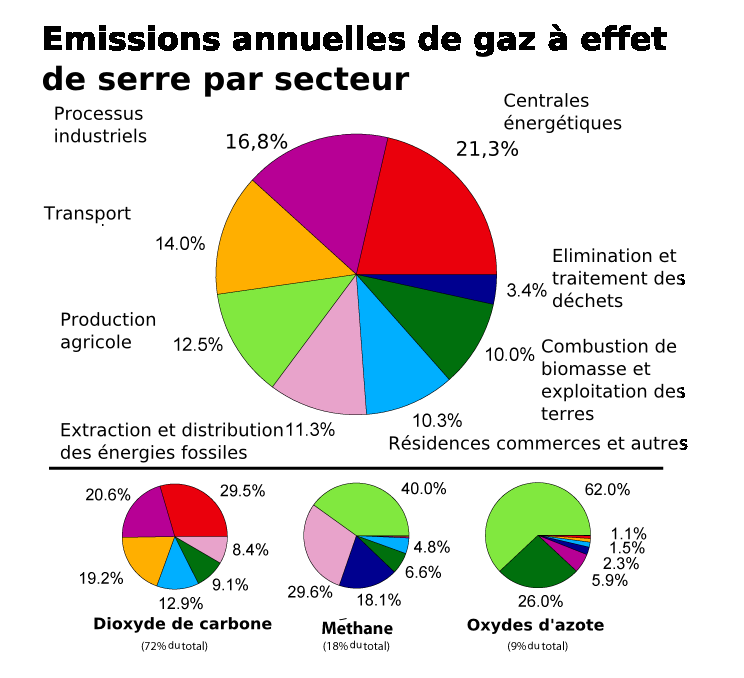
\includegraphics[width=17cm]{Emission_de_GES.png}
Graphique en provenance de l'article \wikipedia{fr}{Gaz_à_effet_de_serre}{gaz à effet de serre} de wikipédia.

\begin{enumerate}
    \item
        Quel est le secteur qui émets le plus ?
    \item
        Est-ce que l'agriculture émet beaucoup de dioxyde de carbone ?
    \item
        À partir des deux graphiques du bas, est-ce que vous êtes capables de retrouver le \( 12.5\%\) de l'agriculture donnés dans le graphique du haut ?
\end{enumerate}

%---------------------------------------------------------------------------------------------------------------------------
\subsection{Découvertes de pétrole}
%---------------------------------------------------------------------------------------------------------------------------

Regardons un instant le graphique suivant, provenant de l'article \wikipedia{fr}{Pic_pétrolier}{Pic pétrolier} de wikipédia.

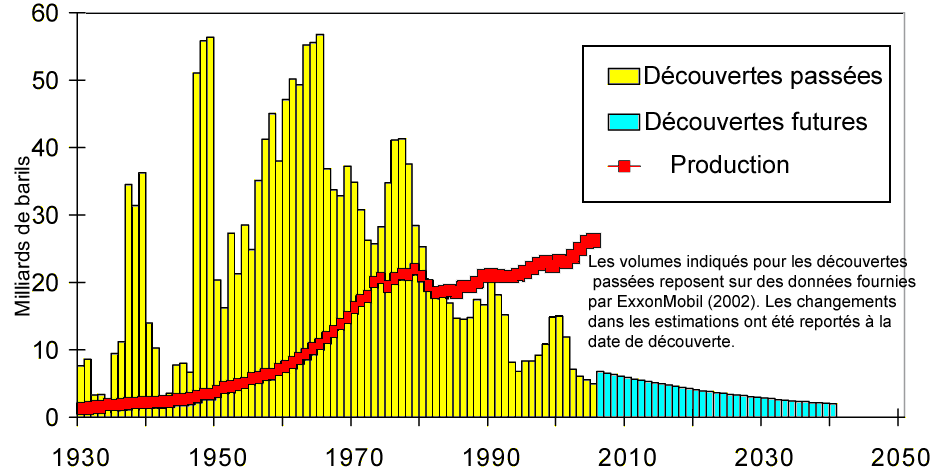
\includegraphics[width=17cm]{Decouvertes-petrole.png}

\begin{enumerate}
    \item
        Quelle est l'année où on a découvert le plus de pétrole ?
    \item
        Quelle est l'année où on a consommé le plus de pétrole ?
    \item
        En quelles années on a consommé autant qu'on a découvert ?
    \item
        Que pensez-vous de l'affirmation «ce qui reste comme réserve est la surface jaune au-dessus de la ligne rouge» ?
\end{enumerate}
Pour aller plus loin, remarquer la cassure assez nette de la croissance de la production vers 1975. Juste par curiosité, faites quelque recherches sur l'histoire de la croissance économique, de la dette publique et le chômage en France (et en Europe). Est-ce que les années 1970 ont été spéciales de ce point de vue ?

%---------------------------------------------------------------------------------------------------------------------------
\subsection{Températures}
%---------------------------------------------------------------------------------------------------------------------------

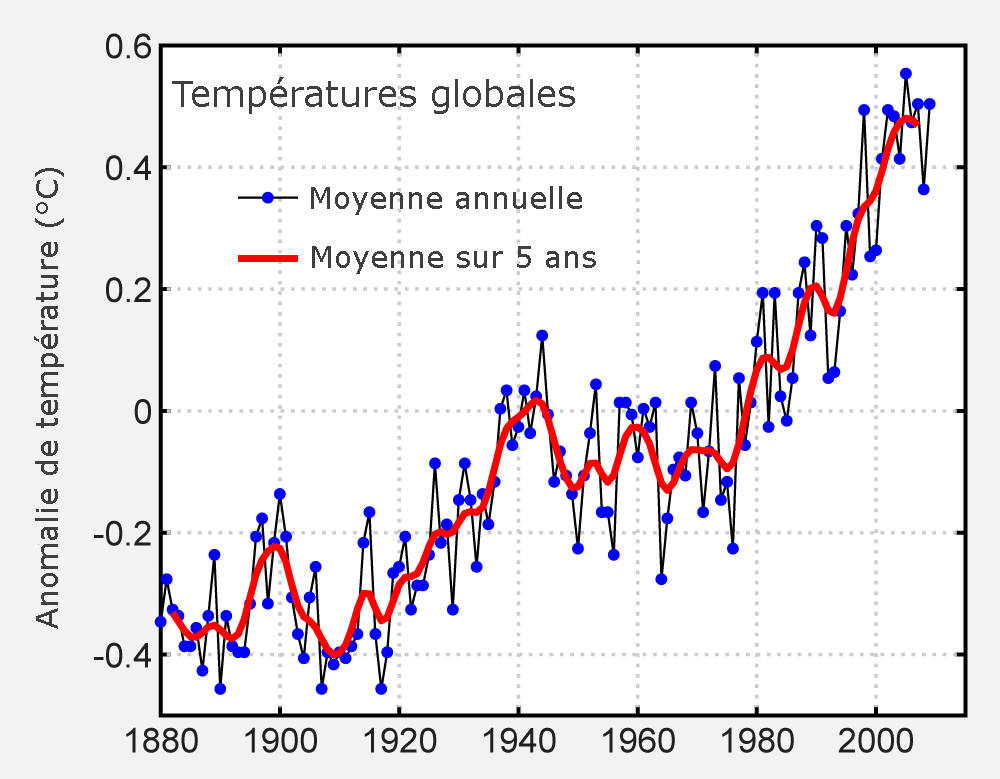
\includegraphics[width=17cm]{Instrumental_Temperature_Record_fr.png}
Graphique en provenance de l'article \wikipedia{fr}{Réchauffement_climatique}{réchauffement climatique} de wikipédia.

Le zéro de ce graphique est la moyenne 1961-1990.

\begin{enumerate}
    \item
        Quelle est la dernière année «normale» ?
    \item
        Quelle est l'année la plus chaude ?
    \item
        Quelle est l'année la plus froide ?
\end{enumerate}

%---------------------------------------------------------------------------------------------------------------------------
\subsection{Consommation de pétrole}
%---------------------------------------------------------------------------------------------------------------------------

Lire le tableau suivant :
\begin{center}
\begin{tabular}[h]{|c|c|c|c|c|c|c|c|c|}
année&
2001&
2002&
2003&
2004&
2005&
2006&
2007&
2008\\
consommation (Mb/j)&
76,8&
77,7&
79,1&
81,8&
83,1&
83,8&
84,9&
84,5
\end{tabular}
\end{center}

Calculer le pourcentage d'augmentation année par année. Que s'est-il passé en 2008 ?

%+++++++++++++++++++++++++++++++++++++++++++++++++++++++++++++++++++++++++++++++++++++++++++++++++++++++++++++++++++++++++++
\section{Théorie}
%+++++++++++++++++++++++++++++++++++++++++++++++++++++++++++++++++++++++++++++++++++++++++++++++++++++++++++++++++++++++++++

\begin{definition}
    Une \defe{population}{population} est un ensemble fini. Une \defe{série statistique}{série statistique} sur une population est une fonction qui à chaque élément (individu) de la population fait correspondre une valeur.

    L'\defe{effectif}{effectif} d'une valeur est le nombre d'individus correspondant à la valeur.

    La \defe{fréquence}{fréquence} d'une valeur est le rapport
    \begin{equation}
        f=\frac{ \text{effectif de la valeur} }{ \text{effectif total} }
    \end{equation}
    où par «effectif total» nous entendons la taille de la population totale.
\end{definition}

La \defe{moyenne}{moyenne} d'une suite de nombres \( x_1,\ldots, x_n\) est
\begin{equation}
    \bar x=\frac{1}{ n }\sum_{i=1}^nx_i=\frac{ \text{somme des \( x_i\)} }{\text{nombre de données}}.
\end{equation}

\begin{example}
    Soit la suite de nombres
    \begin{equation}
        1,7,0,3,9,0,1,3,1,0,2,5,6,9,1,1,3,2,4.
    \end{equation}
    Il y a \( 19\) nombres. La moyenne est donnée par la fraction
    \begin{equation}
        \bar x=\frac{ 1+7+0+3+9+\ldots+3+2+4 }{ 19 }=\frac{ 58 }{ 19 }.
    \end{equation}

Python permet d'obtenir assez facilement une approximation numérique :
    \begin{verbatim}
>>> import numpy
>>> nombres=[1,7,0,3,9,0,1,3,1,0,2,5,6,9,1,1,3,2,4]
>>> numpy.mean(nombres)          # 'mean' signifie 'moyenne' en anglais.
3.0526315789473686 
    \end{verbatim}
\end{example}

\begin{example}
    Voici un petit tableau de l'\href{http://www.insee.fr/fr/themes/tableau.asp?reg_id=0&ref_id=NATTEF13325}{INSEE}, parlant du chiffre d'affaire des éditeurs vidéos en million d'euros.

    \begin{center}
    \begin{tabular}{|c|c|c|c|c|c|}
        \hline
        &Vidéo à la demande &   \multicolumn{3}{| c |}{Vente}&Total\\
        \hline
        &                   &   total&dont DVD&dont Blu-ray&\\
        \hline
        2004&nd&1958.8&1844.6&&nd\\
        2005&nd&1784.2&1757.3&&nd\\
        2006&nd&1659.2&1654.7&&nd\\
        2007&28.9&1494.1&1479.9&14.3&1523.0\\
        2008&53.2&1382.4&1331.0&51.5&1435.6\\
        2009&97.0&1384.4&1277.1&107.3&1481.4\\
        2010&152.0&1385.4&1211.7&173.7&1537.4\\
        2011&219.5&1257.5&1048.4&209.1&1477\\
        \hline
    \end{tabular}
    \end{center}
    Dessiner un diagramme en camembert pour les années 2007 et 2011.
\end{example}



\newcommand{\comp}{{\ \ldots\ldots\ }} %
\newcommand{\exe}[1]{\par \smallskip %
  \fontfamily{cmss}\selectfont Exemple : \  \normalfont%
  \begin{minipage}[t]{0.8\linewidth}%
    \textit{#1}%
  \end{minipage} \par%
  \medskip
}

%\documentclass[french,a4paper,12pt]{book}
%\input{../Macros}
%\geometry{vmargin=40pt,hmargin=40pt}
%% -------------------------------
%% Repertoire de figures
%\graphicspath{{Cours_Statistiques/}}  
%% -------------------------------
%\input{Macros_Cours}
%
%\begin{document}
%
%
%
%
%\setlength{\baselineskip}{16pt}
%
%\setcounter{chapter}{5}
%%\setcounter{section}{2}
%%\setcounter{subsection}{1}
%
%\newcommand{\voc}[1]{\fontfamily{ppl}\selectfont #1\normalfont}
%\newcommand{\voc}[1]{\fontfamily{cmss}\selectfont #1\normalfont}

%\newcommand{\rmq}[1]{\par \medskip %
%  \fontfamily{cmss}\selectfont \noindent Remarque : \  \normalfont%
%  \begin{minipage}[t]{0.89\linewidth} 
%    #1 
%  \end{minipage} \par%
%  \medskip
%}
%}
%\newcommand{\para}[1]{\par \medskip%
%  \fontfamily{cmss}\selectfont \noindent #1 %
%  \normalfont %
%}
%\newcommand{\parag}[2]{\par \medskip %
%  \fontfamily{cmss}\selectfont \noindent #1 \  \normalfont%
%  \begin{minipage}[t]{0.84\linewidth} 
%    #2
%  \end{minipage} \par%
%  \medskip
%}
%\newcommand{\paragit}[2]{\par \medskip %
%  \fontfamily{cmss}\selectfont \noindent #1 \  \normalfont%
%  \begin{minipage}[t]{0.84\linewidth} 
%    \textit{#2}
%  \end{minipage} \par%
%  \medskip
%}
%
%\newcommand{\definition}[1]{\par \medskip %
%  \fontfamily{cmss}\selectfont \noindent Définition : \\[2pt] 
%  \normalfont%
%  \fbox{
%    \begin{minipage}[t]{0.95\linewidth} #1 \end{minipage} \par%
%    \medskip
%  }    \medskip
%}
%%\let\DEFINITION=\definition
%%\renewenvironment{definition}{\DEFINITION\bgroup}{\egroup}
%




% %%%%%%%%%%%%%%%%%%%%%%%%%%%%%%%%%%%%%%%%%%%%%
%    DEBUT DU COURS
% %%%%%%%%%%%%%%%%%%%%%%%%%%%%%%%%%%%%%%%%%%%%%


Le rôle de la statistique descriptive est de présenter une masse de
données sous forme lisible, puis, si possible, de la résumer par
quelques nombres caractéristiques (moyenne, médiane, etc.).



% %%%%%%%%%%%%%%%%%%%%%%%%%%%%%%%%%%%%%%%%%%%%%
%    VOCABULAIRE
% %%%%%%%%%%%%%%%%%%%%%%%%%%%%%%%%%%%%%%%%%%%%%

\section{Vocabulaire}

\begin{enumerate}
    \item La \defe{population}{} désigne l'ensemble des personnes ou objets,
  aussi appelés individus, sur lesquels porte l'étude
  statistique.  
  \exe{Les élèves de la classe de 2\up{nde}B, les habitants d'un pays,
    les voitures produites en 2010, les employés d'une entreprise.}
\item On recueille alors des données concernant un \defe{caractère}{} sur
  les individus de cette population. Ce caractère peut prendre un
  certain nombre de \defe{valeurs}{}, numériques ou non.
  \exe{La taille des élèves de la classe, le salaire des employés, la
  couleur des voitures construites.}
\item Un caractère est dit \defe{quantitatif}{} lorsqu'il est possible de
  le mesurer en associant un nombre à chaque individu. Dans ce cas, le
  caractère quantitatif est aussi appelé \defe{variable}{}.
  \exe{L'âge, la taille, le nombre d'enfants dans une famille.}
  \begin{enumerate}
      \item Un caractère quantitatif est dit \defe{continu}{} lorsque les
    nombres qui le mesurent peuvent prendre a priori toutes les
    valeurs d'un intervalle.
    \exe{La taille, un salaire, la durée de vie d'un baladeur.}
\item Le caractère est dit \defe{discret}{} dans le cas contraire.
    \exe{L'année de naissance, le nombre de frères et soeurs.}
  \end{enumerate}
\item On appelle caractère \defe{qualitatif}{} tout caractère qui n'est
  pas quantitatif.
  \exe{La couleur des yeux, le chanteur préféré, le choix de la
    section de 1\up{ère}.} 
\end{enumerate}


\begin{example}
Une revue présente un tableau donnant les prix en euros d'appareils photos numériques.

  \begin{center}

    \begin{tabular}[t]{|l|c|c|c|c|}
      \hline
      \textbf{Prix} & $[300;500[$ & $[500;700[$ & $[700;900[$ &
      $[900;1\,100[$ \\
      \hline
      \textbf{Effectif} & 14 & 8 & 3 & 1 \\
      \hline
    \end{tabular}
      
  \end{center}

  \begin{enumerate}
  \item Quelle est la population étudiée ? \\[1ex]
  \item Quel est le nombre d'individus de cette population ?\\[1ex]
  \item Quel est le caractère ? \\[1ex]
  \item Ce caractère est-il quantitatif ?
  \end{enumerate}
  
\end{example}

% %%%%%%%%%%%%%%%%%%%%%%%%%%%%%%%%%%%%%%%%%%%%%
%    PRÉSENTATION D'UNE SÉRIE
% %%%%%%%%%%%%%%%%%%%%%%%%%%%%%%%%%%%%%%%%%%%%%

\section{Présentation des éléments d'une série statistique}

\subsection{Effectifs. Effectifs cumulés croissants}

On donne souvent une série statistique par un tableau d'effectifs.

\begin{example} \label{ExUDXDZl}
Dans un village, on recense le nombre d'enfants par foyer; le résultats est donné dans le tableau suivant.

\begin{center}
\begin{tabular}[h]{|c|c|c|c|c|c|c|c|c|}
    \hline
  \textbf{Nombre d'enfants $x_i$} & 0 & 1 & 2 & 3 & 4 & 5 & 6 & 7 \\
  \hline
  \textbf{Effectif $n_i$} & 290 & 170 & 155 & 95 & 43 & 27 & 20 & 10\\
  \hline
\end{tabular}
\end{center}

Dans ce tableau nous lisons que \( 155\) foyers ont 2 enfants.
    
\end{example}

On note généralement $n$ l'\defe{effectif total}{}, $n=n_1+n_2+n_3+{\ldots}+n_8$. 

\textit{Ici, l'effectif total vaut :  \comp. }

Le \defe{mode}{} est la valeur ayant le plus grand effectif. Elle a un intérêt si l'effectif de cette valeur est nettement plus grand que les autres effectifs. Il peut y avoir plusieurs modes si plusieurs valeurs ont les mêmes effectifs.

\textit{Dans cet exemple, le mode est égal à \comp.}

À partir du tableau, on peut dresser le tableau des \defe{effectifs cumulés croissants}{}.

\begin{example} \label{ExZdeBXW}
    Nous continuons l'exemple \ref{ExUDXDZl} en ajoutant la ligne des effectifs cumulés.
\begin{center}
\begin{tabular}[h]{|c|c|c|c|c|c|c|c|c|}
    \hline
  \textbf{Nombre d'enfants $x\leq$} & 0 & 1 & 2 & 3 & 4 & 5 & 6 & 7 \\
  \hline
  \textbf{Effectif $n_i$} & 290 & 170 & 155 & 95 & 43 & 27 & 20 & 10 \\
  \hline
  \textbf{Effectif cumulé croissant} & 290 & 460 & 615 & 710 & 753 & 780 & 800 & 810 \\ 
  \hline
\end{tabular}
    
\end{center}

Dans ce tableau, nous lisons  que le nombre d'enfants est inférieur ou égal à 2 dans 615 foyers.
    
\end{example}



\begin{remark}
Le tableau des effectifs cumulés donne directement le nombre de foyers qui ont au plus $x_i$ enfants.  Par exemple, pour $x_i=5$, il y a \( 780\) foyers qui ont au plus 5 enfants.
\end{remark}


\begin{remark}
Le tableau des effectifs cumulés permet également de repérer facilement la $n$-ième valeur donnée de la série triée par ordre croissant.  Par exemple, le $750$\ieme{} foyer correspond à un foyer ayant \( 4\) enfants. 
\end{remark}


\subsection{Fréquences. Fréquences cumulées croissantes}

À partir des effectifs, on peut dresser le tableau des fréquences.

Par définition, la \defe{fréquence}{} d'une valeur du caractère $x_i$ est :
\[
\mbox{fréquence} 
= \frac{\mbox{effectif $n_i$ du caractère}}{\mbox{effectif total}}
\qquad
\mbox{soit} 
\qquad
f_i = \dfrac{n_i}{n}
\]

\begin{example}
Nous continuons l'exemple \ref{ExUDXDZl}, $f_1 = \dfrac{n_1}{n} = \dfrac{290}{810} \approx 0,36$. Cela signifie que parmi les foyer, une proportion de \( 0.36\) (\( =36\%\)) a exactement un enfant. Les autres résultats sont dans le tableau suivant.

\begin{center}
\begin{tabular}[t]{|c|c|c|c|c|c|c|c|c|}
    \hline
  \textbf{Valeur $x_i$} & 0 & 1 & 2 & 3 & 4 & 5 & 6 & 7 \\
  \hline
  \textbf{Fréquence $f_i$} & 0,36 & 0,21 & 0,19 & 0.12  & 0.05 & 0.03 & 0.02 & 0.01 \\ 
  \hline
\end{tabular}
    
\end{center}
    
\end{example}


Les fréquences vérifient les propriétés suivantes :
\begin{enumerate}
  \item Une fréquence est toujours comprise entre 0 et 1 :
      \begin{equation}
    0\leq f_i\leq 1.
      \end{equation}
  \item La somme des fréquences est toujours égale à 1.  
      \begin{equation}
      f_1+f_2+{\ldots}+f_8 =  1.
      \end{equation}
\end{enumerate}

\bigskip

À partir du tableau des fréquences, on peut dresser le tableau des \defe{fréquences cumulées croissantes}{}, en ajoutant à chaque fréquence la somme des fréquences précédentes\footnote{Notons que les erreurs d'arrondi font en sorte que le dernier saut ne tombe pas juste. De toutes façons, la dernière case doit être \( 1\).}.

\begin{center}
\begin{tabular}[h]{|c|c|c|c|c|c|c|c|c|}
    \hline
  \textbf{Valeur $x_i$} & 0 & 1 & 2 & 3 & 4 & 5 & 6 & 7 \\
  \hline
  \textbf{Fréquence $f_i$} & 0,36 & 0,21 & 0,19 & 0,12 & 0.05  & 0.03 & 0.02 & 0.01 \\ 
  \hline
  \textbf{Fréquence cumulée croissante} & 0,36 & 0,57 & 0,76 & 0.88 & 0.93 & 0.96 & 0.98  & 1 \\ 
  \hline
\end{tabular}
\end{center}

 À partir du tableau des fréquences cumulées, on lit que \( 76\) \% des foyers ont moins de 3 enfants, et \( 88\)\% des foyers ont moins de 4 enfants.

\subsection{Représentation en classes}

Lorsque les valeurs étudiées sont en très grand nombre, on peut les
regrouper dans des intervalles de la forme $[a;b[$ appelés
    \defe{classes}{}. 

    L'\defe{amplitude}{} de la classe est $b-a$, c'est l'écart entre la plus
grande et la plus petite valeur de la classe.

Le \defe{centre}{} de la classe est la moyenne $\dfrac{a+b}2$.

La \defe{classe modale}{} est la classe qui a le plus grand effectif. 

\medskip

\begin{example}
Le tableau ci-dessous donne la répartition des masses de nouveaux-nés dans un hôpital, de 2,5 $kg$ à 4,5 $kg$.


\begin{center}
  \begin{tabular}[h]{|l|c|c|c|c|}
    \hline
    \textbf{Masse en kg} & $[2,\!5\,;3[$ & $[3\,;3,\!5[$ & $[3,\!5\,;4[$ &
    $[4\,;4,\!5[$ \\
    \hline
    \textbf{Effectif} & 15 & 32 & 40 & 13 \\
    \hline
  \end{tabular}
    
\end{center}
  
De ce tableau, nous tirons :
\begin{enumerate}
    \item
  l'effectif total est égal à \( 100\);
  \item
  l'amplitude des classes est égale à \( 0.5\);
  \item
  le centre de la deuxième classe est \( 3.25\);
  \item
  la classe modale est la troisième.
\end{enumerate}


    
\end{example}


% %%%%%%%%%%%%%%%%%%%%%%%%%%%%%%%%%%%%%%%%%%%%%
%    VALEURS CARACTERISTIQUES
% %%%%%%%%%%%%%%%%%%%%%%%%%%%%%%%%%%%%%%%%%%%%%

\renewcommand{\exe}[1]{\par %\smallskip %
  \noindent%
  \fontfamily{cmss}\selectfont Exemple : \  \normalfont%
  \begin{minipage}[t]{0.85\linewidth}%
    \textit{#1}%
  \end{minipage} \par%
  \medskip
}

\section{Étude d'une série statistique : grandeurs caractéristiques}

On considère une série statistique dont les valeurs du caractère sont
$x_1$, $x_2$, {\ldots}, $x_p$, et les effectifs correspondants :
$n_1$, $n_2$, {\ldots}, $n_p$.

%\bigskip
%\medskip


\subsection{Moyenne}

\begin{definition}
    La \defe{moyenne}{} de la série statistique des $(x_i;n_i)$ est le
  nombre, noté $\overline{x}$, défini par
  \[
  \overline{x} =
  \frac{n_1x_1+n_2x_2+{\ldots}+n_px_p}{n} 
  \]
  où $n = n_1+n_2+{\ldots}+n_p$ est l'effectif total.

    
\end{definition}

\bigskip


\exe{On reprend le tableau 1 donnant le nombre d'enfants par foyer
  dans un village. Dans ce village, le nombre moyen d'enfants par
  foyer est  
\begin{align*}
  \overline{x} = {} & 
  \frac{290\times0+170\times1+155\times2+95\times
    3+43\times 4+27\times 5+20\times 6+10\times 7}{810}
  \\[1ex]
  \overline{x} \approx {} & 1,6
\end{align*}
}
\medskip

\begin{remark}
On peut aussi calculer $\overline{x}$ en utilisant les fréquences
  $f_i$ : \\[1ex]
  $ \overline{x} = f_1 x_1 + f_2x_2+{\ldots}+f_px_p $. 

    
\end{remark}

\subsection{Médiane}

\begin{definition}
    La \defe{médiane}{}, notée $M_e$, d'une série statistique est un
  nombre qui partage la population en deux parties :
  \begin{enumerate}
  \item 50 \% au moins des individus ont une valeur du caractère
    inférieure ou égale à $M_e$ ;
  \item 50 \% au moins des individus ont une valeur du caractère
    supérieure ou égale à $M_e$.
  \end{enumerate}  

    
\end{definition}


\paragraph{En pratique :}On range les $n$ valeurs de la série par ordre
  croissant, chacune étant répétée autant de fois que son effectif.


\begin{enumerate}
\item Si $n$ est impair, la médiane est la valeur centrale de la série ;
\item Si $n$ est pair, la médiane est la demi-somme des deux valeurs
  centrales de la série.
\end{enumerate}

%\bigskip
\medskip

\begin{example}
\begin{enumerate}
\item Pour une série de 7 valeurs rangées par ordre
    croissant, la médiane est la quatrième valeur (il y en a \( 3\) à gauche et \( 3\) à droite).
\item Si la série comporte 12 valeurs, la médiane est la moyenne entre la sixième et la septième valeur (il y en a alors \( 5\) à gauche et \( 5\) à droite)
\item Si la série comporte 6 valeurs, la médiane est la moyenne ente la moyenne entre la troisième et la quatrième valeur. 
\item Si la série comporte 25 valeurs, la médiane est la treizième valeur.
\item Si la série comporte 15 valeurs, la médiane est la huitième valeur.
\end{enumerate}
    
\end{example}

\paragraph{Application :}Dans chaque cas, déterminer la médiane de la
  série.\\
  Conseil : on commencera par trier les valeurs de la série par ordre
  croissant, et on donnera l'effectif total.


\begin{enumerate}
\item 5 ; 10 ; 17 ; 12 ; 6 
\item 1\,000 ; 1\,000 ; 1\,200 ; 1\,200 ; 1\,200 ; 1\,500 ; 1\,500 ;
  2\,000 ; 2\,500 ; 3\,100 
\item 5 ; 1 ; 2 ; 9 ; 4 ; 5 ; 7 ; 5 ; 9 ; 5 ; 6 ; 7 ; 8 ; 9 ; 2 ; 9 ;
  6 ; 5 ; 9 ; 3 
\end{enumerate}

\begin{remark}
La médiane ne dépend pas des valeurs extrêmes.
\end{remark}

\begin{example}
    Comment manipuler des chiffres et la perception des coefficients des épreuves du bac. en utilisant à tort et à travers la notion de moyenne ?\\
    \url{http://allken-bernard.org/pierre/weblog/?p=2386}
\end{example}

\subsection{Quartiles}

\begin{definition}
  On considère une liste de $n$ valeurs, \underline{triées par ordre
    croissant}. 
  \begin{enumerate}
      \item Le \defe{premier quartile}{} $Q_1$ est la plus petite valeur de
    la liste telle qu'au moins un quart des valeurs de la liste sont
    inférieures ou égales à $Q_1$.
\item Le \defe{troisième quartile}{} $Q_3$ est la plus petite valeur de
    la liste telle qu'au moins les trois quarts des valeurs de la
    liste sont inférieures ou égales à $Q_3$.
  \end{enumerate}

    
\end{definition}


En pratique :
\begin{itemize}
    \item 
  Pour le calcul de $Q_1$, on calcule $\dfrac{n}4$, puis on détermine
  le premier entier $p$ supérieur ou égal à $\dfrac{n}4$. Cet entier
  $p$ donne le rang de $Q_1$. 
  \item
  Pour le calcul de $Q_3$, on fait de même en remplaçant $\dfrac{n}4$
  par $\dfrac{3n}4$. 
\end{itemize}

Du point de vue de la programmation, python a la fonction \info{math.ceil} pour calculer le premier entier supérieur ou égal à \( p\).

\lstinputlisting{exemple_ceil.py}

  \begin{example}
  \begin{enumerate}
  \item Pour $n=15$, on a \ $\dfrac{n}4 = 3,75$, donc $Q_1$ est la
    4\ieme{} valeur de la série (lorsqu'elle est rangée par ordre
    croissant). 
    De plus, \( \frac{ 3 }{ 4 }15=11.25\), donc $Q_3$ est la 12\up{e} valeur de la
    série. 
  \item Pour $n=18$, $Q_1$ est la 5\up{e} valeur (\( 18/4=4.5\)), et $Q_3$ est la 14\up{e} valeur de la série.
\end{enumerate}
      
  \end{example}

\subsection{Mesures de dispersion}


\begin{enumerate}
    \item L'\defe{étendue}{} d'une série statistique est la différence entre
  la plus grande et la plus petite valeur.
\item L'\defe{écart interquartile}{} est égal à la différence $Q_3-Q_1$.
\end{enumerate}


\begin{example}
Pour la série  1\,000 ; 1\,000 ; 1\,200 ; 1\,200 ; 1\,200 ; 1\,500 ; 1\,500 ;
  2\,000 ; 2\,500 ; 3\,100 ; étudiée ci-dessus, 
  \begin{enumerate}
  \item l'étendue vaut \( 3100-1000=2100\),
  \item l'écart interquartile est égal à \( 2000-1200=800\).
  \end{enumerate}
\end{example}

\subsection{Lecture des grandeurs caractéristiques à l'aide des
  effectifs cumulés croissants}

  \begin{example}

À partir du tableau suivant, nous pouvons trouver les quartiles en ne lisant que la ligne des effectifs cumulés.

  \begin{center}
\begin{tabular}[h]{|c||c|c|c|c|c|c|c|c|c|c|c|}
    \hline
  \textbf{Valeur} & 73 & 74 & 75 & 76 & 77 & 78 & 79 & 80 & 81 & 82 & 83 \\
  \hline
  \textbf{Effectif} & 2 & 4 & 3 & 7 & 9 & 6 & 8 & 3 & 4 & 2 & 2 \\ 
  \hline
  \textbf{Eff. cum. cr.} & 2 & 6 & 9 & 16 & 25 & 31 & 39 & 42 & 46 & 48 & 50 \\ 
  \hline
\end{tabular}
      
  \end{center}

D'abord la dernière case nous dit que l'effectif total est égal à \( 50\). Nous en déduisons que
\begin{enumerate}
  \item Le premier quartile est la 13\up{e} valeur.
  \item La médiane est la moyenne entre la 25\up{e} et la 26\up{e} valeurs.
  \item Le troisième quartile est la 38\up{e} valeur.
\end{enumerate}
La première case des effectifs cumulés à être plus grande (ou égale) à \( 13\) est la case du \( 76\); le premier quartile est donc égal à \( 76\).

Pour la médiane, la \( 25\)\up{e} et la \( 26\)\up{e} sont toutes deux égales à \( 77\); donc la médiane est \( 77\).

En ce qui concerne le troisième quartile, la \( 38\)\up{e} valeur est \( 79\).

\begin{subequations}
    \begin{align}
        Q_1&=76\\
        M_e&=77\\
        Q_2&=79.
    \end{align}
\end{subequations}
  \end{example}

\subsection{Lecture des quartiles à l'aide des fréquences cumulées croissantes}

Dans le tableau des fréquences cumulées croissantes :
\begin{enumerate}
\item le premier quartile $Q_1$ est la première valeur de la série
  pour laquelle la fréquence cumulée croissante $0,25$ est atteinte ou
  dépassée ;
\item le troisième quartile $Q_3$ est la première valeur de la série
  pour laquelle la fréquence cumulée croissante $0,75$ est atteinte ou
  dépassée.
\end{enumerate}


\begin{center}
\begin{tabular}[h]{|c||c|c|c|c|c|c|c|c|c|c|c|}
    \hline
  \textbf{Valeur} & 73 & 74 & 75 & 76 & 77 & 78 & 79 & 80 & 81 &
  82 & 83 \\
  \hline
%  \cline{1-12}
%  \textbf{Effectif} & 2 & 4 & 2 & 7 & 9 & 6 & 8 & 3 & 4 & 2 & 2 &\\ 
%   \cline{1-12}
%   \textbf{Effectif cumulé} & 2 & 6 & 9 & 16 & 25 & 31 & 39 &
%   42 & 46 & 48 & 50 &\\ 
  \textbf{Freq. cum. cr.} & 0,04 & 0,12 & 0,18 & 0,32 & 0,50 & 0,62 & 0,78 &
  0,84 & 0,92 & 0,96 & 1 \\ 
  \hline
\end{tabular}
\end{center}

Le premier quartile vaut $Q_1=76$. Le troisième quartile vaut \ $Q_3=79$. L'écart interquartile vaut alors \( 79-76=3\).


% %%%%%%%%%%%%%%%%%%%%%%%%%%%%%%%%%%%%%%%%%%%%%
%    REPRESENTATION GRAPHIQUE
% %%%%%%%%%%%%%%%%%%%%%%%%%%%%%%%%%%%%%%%%%%%%%

\section{Représentation graphique d'une série statistique}

%TODO : le diagramme en boîte n'est pas au programme de seconde. Il faut donc l'enlever.

\begin{multicols}{2}
\subsection{Nuage de points}
  \begin{enumerate}
  \item En abscisses, les valeurs du caractère.
  \item En ordonnées, les effectifs (ou les fréquences)
  \end{enumerate}
  \columnbreak
  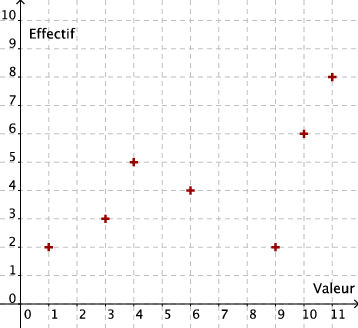
\includegraphics[width=5cm]{Stats_Fig4_Nuage.png}
\end{multicols}

\subsection{Diagramme en bâtons, ou diagramme en barres}

\begin{multicols}{2}
\begin{enumerate}
\item Pour des caractères qualitatifs.
\item L'abscisse représente les valeurs.
\item La hauteur du bâton est proportionnelle à l'effectif (ou à la fréquence).
\end{enumerate}

\exe{V{\oe}u d'orientation des élèves d'une classe de seconde}
\columnbreak
  \begin{center}
    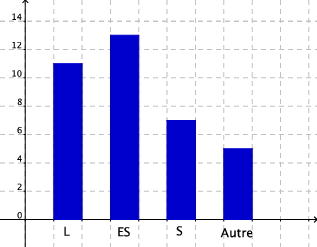
\includegraphics[width=6cm]{Stats_Fig4_DiagBaton.png}
  \end{center}    
\end{multicols}

\subsection{Histogramme}

\begin{enumerate}
\item Pour des données rassemblées en classes
\item L'\textbf{aire} du rectangle est proportionnelle à l'effectif (ou à la
fréquence). 
\end{enumerate}

\begin{multicols}{2}
  \begin{center}
    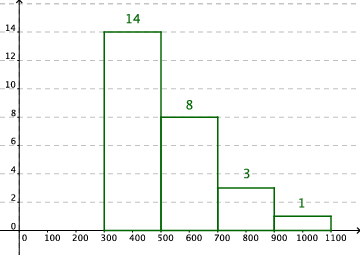
\includegraphics[width=6cm]{Stats_Fig4_HistPC.png}
    Histogramme à pas constant \\
    (classes de même amplitude)     
  \end{center}

  \columnbreak

  \begin{center}
    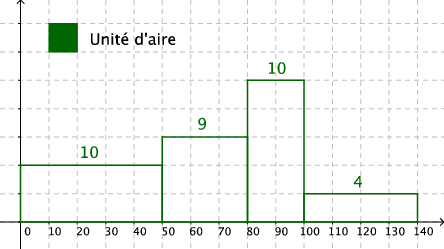
\includegraphics[width=6cm]{Stats_Fig4_HistPNC.png}
    Histogramme à pas non constant \\
    (classes d'amplitudes différentes)
  \end{center}
  
\end{multicols}

Consignes pour dessiner un histogramme :
\begin{enumerate}
    \item
        Trouver la plus haute boite en calculant le rapport \( \frac{ \text{effectif} }{ \text{largeur} }\) pour chaque boite.
    \item
        Se fixer une échelle pour que la plus haute boite reste raisonnable : elle ne doit pas faire deux mètres de haut, ni un centimètre. Il faut viser environ \unit{10}{\centi\meter}.
    \item
        Tracer les boites.
    \item
        Mettre la graduation \emph{horizontale} en écrivant la légende correspondante.
    \item
        Ne pas mettre de graduation verticale en cas d'histogramme à pas non constant\footnote{C'est à dire ceux dont la largeur n'est pas la même pour toute les boites.}.
    \item
        Écrire l'effectif de la boite au-dessus de la boite.
    \item
        Éventuellement écrire l'unité de surface «un carreau= \ldots effectifs». Par exemple «un carreau = 50 entreprises», «un carreau = 15 personnes».
\end{enumerate}
Voir la correction de l'exercice \ref{exoSeconde-0033} pour un exemple détaillé.

\subsection{Diagramme circulaire}

\begin{multicols}{2}
  \begin{enumerate}
  \item L'angle au centre du secteur circulaire est proportionnel à l'effectif
    de chaque valeur.
  \end{enumerate}
  
  
  \exe{Production de fromages en France, en milliers de tonnes
  }
  \columnbreak
  \begin{minipage}{1.0\linewidth}
    \vspace{-2em}
    \begin{center}
      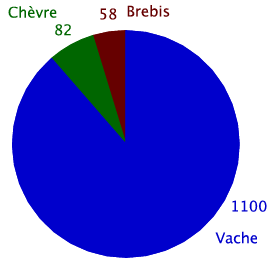
\includegraphics[width=5cm]{Stats_Fig4_DiagCirc.png}
    \end{center}    
  \end{minipage}
\end{multicols}



\subsection{Diagramme des effectifs/fréquences cumulé(e)s croissant(e)s}

\begin{multicols}{2}
  \begin{center}
    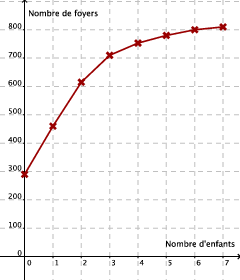
\includegraphics[width=6cm]{Stats_Fig4_DiagEffCum.png}
    
    Diagramme des effectifs cumulés croissants    
  \end{center}

  \columnbreak
  \begin{center}
    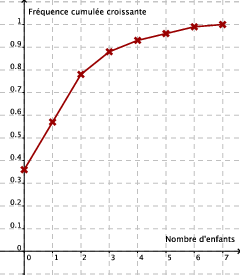
\includegraphics[width=6cm]{Stats_Fig4_DiagFreqCum.png}

    Diagramme des fréquences cumulées croissantes
  \end{center}
\end{multicols}



\subsection{Diagramme en boîte, ou diagramme à moustaches}

\begin{enumerate}
\item Pour des séries ayant un grand nombre de valeurs
\item Basé sur les quartiles et la médiane
\end{enumerate}

\begin{center}
  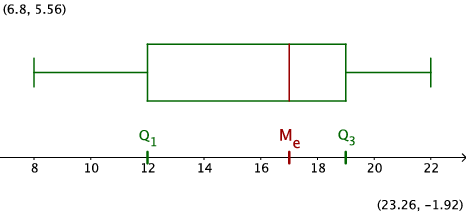
\includegraphics[width=7cm]{Stats_Fig4_DiagBoite.png}  
\end{center}




%+++++++++++++++++++++++++++++++++++++++++++++++++++++++++++++++++++++++++++++++++++++++++++++++++++++++++++++++++++++++++++
\section{Exercices}
%+++++++++++++++++++++++++++++++++++++++++++++++++++++++++++++++++++++++++++++++++++++++++++++++++++++++++++++++++++++++++++

%---------------------------------------------------------------------------------------------------------------------------
\subsection{Proportions, pourcentage}
%---------------------------------------------------------------------------------------------------------------------------

\Exo{Seconde-0023}
\Exo{Seconde-0031}
\Exo{Seconde-0025}
\Exo{smath-0296}

%---------------------------------------------------------------------------------------------------------------------------
\subsection{Moyenne}
%---------------------------------------------------------------------------------------------------------------------------

\Exo{Seconde-0039}
\Exo{smath-0011}
\Exo{smath-0012}
\Exo{smath-0250}
\Exo{smath-0315}

%---------------------------------------------------------------------------------------------------------------------------
\subsection{Médiane, quartiles}
%---------------------------------------------------------------------------------------------------------------------------

\Exo{Seconde-0029}
\Exo{Seconde-0027}
\Exo{Seconde-0028}
\Exo{smath-0147}
\Exo{Seconde-0014}
\Exo{Seconde-0032}
\Exo{Seconde-0015}
\Exo{Seconde-0037}
\Exo{Seconde-0016}
\Exo{Seconde-0017}
\Exo{Seconde-0073}
\Exo{Seconde-0074}

%---------------------------------------------------------------------------------------------------------------------------
\subsection{Histogrammes}
%---------------------------------------------------------------------------------------------------------------------------

\Exo{Seconde-0033}
\Exo{Seconde-0035}
\Exo{Seconde-0036}
\Exo{Seconde-0038}

\Exo{Seconde-0040}


